\documentclass[12pt, a4]{report}
\usepackage[utf8]{inputenc}
\usepackage[margin=0.8in]{geometry}
\def\thesection{\arabic{section}}
\setcounter{tocdepth}{4}
\usepackage{graphicx}
\graphicspath{ {images/} }
% Below are for the code blocks
\usepackage{listings}
\usepackage{courier}
\usepackage{verbatim}
\usepackage{color}
\usepackage{rotating}

% Below are table config
\setlength{\arrayrulewidth}{0.5mm}
\setlength{\tabcolsep}{10pt}
\renewcommand{\arraystretch}{1.5}

\definecolor{codegreen}{rgb}{0,0.6,0}
\definecolor{codegray}{rgb}{0.5,0.5,0.5}
\definecolor{codepurple}{rgb}{0.58,0,0.82}
\definecolor{backcolour}{rgb}{0.95,0.5,0.92}
\definecolor{bittersweet}{rgb}{1.0, 0.44, 0.37}
\definecolor{cosmiclatte}{rgb}{0.93, 0.93, 0.93}
\definecolor{eggshell}{rgb}{0.94, 0.94, 0.9}
\definecolor{fandango}{rgb}{0.71, 0.2, 0.54}

\lstdefinestyle{mystyle}{
	backgroundcolor=\color{cosmiclatte},   
	commentstyle=\color{codegreen},
	keywordstyle=\color{fandango}\small,
	numberstyle=\tiny\color{codegray},
	stringstyle=\color{codepurple},
	basicstyle=\ttfamily\footnotesize,
	breakatwhitespace=false,        
	breaklines=true,               
	captionpos=b,                    
	keepspaces=true,  
	numbers=left,                    
	numbersep=5pt,                  
	showspaces=false,                
	showstringspaces=false,
	showtabs=false,                  
	tabsize=2
}

\lstset{style=mystyle}

\title{2805ICT, Milestone 2: Progress Report}
\author{Natnicha Titiphanpong, s2940970}%\thanks{}}
\date{\today}

\begin{document}
\begin{titlepage}
	\maketitle 
\end{titlepage}
	\tableofcontents
	\pagebreak
	\section{Progress Report} 
	\subsection{Requirements}
	\par The current  version of minesweeper successfully meets the requirements of the traditional minesweeper game however it is still yet to implement the hexagon and colour-based minesweeper  modes successfully. 
		\subsubsection{List of completed requirements}
		Functionality associated with icons |
		The program is able to meet this requirements by accomplishing the following actions:
		\begin{itemize}
			\item The program shows whether a cell is covered or uncovered by clearly displaying the state of the buttons. The buttons possess a 3D-like image when unclicked, the colour of the buttons change once it is sunken (or clicked) into a darker contrast of the same colour. 
			\item When a cell with no adjacent mines is clicked, all adjacent cells alike are uncovered until it reaches a cell with adjacent mines. This task was done in a while loop, not recursively (as there was no need) as previously stated. 
			\item The state of the board, once the buttons are pressed, are represented by a 'backing grid' which assigns all cells with a number or mine, according to the randomly generated mines and its coordinates.
			\item The program displays whether a cell has a mine or not by representing it with an image of a mine when pressed and also displaying a message that the game is over.
		\end{itemize}
f		\newline
		Displaying icons |
		\begin{itemize}
		\par
		\item The program uses the tkinter module and its button component. This makes responding to left mouse click for icon display possible. The left click implementation for the flag is yet to be implemented. 
		\end{itemize}
		Losing a game |
		\begin{itemize}
		\par 
		\item When the user clicks on a button which reveals a mine, a message is displayed in the window "Game Over!" and the state of the game is disabled. 
		\end{itemize}
		Options |
		\begin{itemize}
		\par 
		\item The user is able to start the game by selecting a difficulty and not a game mode, the program will default to the basic minesweeper game. 
		\item Selecting the cross at the top right of the window will exit the program and window. 
		\end{itemize}
		Flagging | 
		\begin {itemize}
		\item The user is able to flag a cell that they believe is a mine.
		\item If all mines are flagged, the game is won.
		\end{itemize}
			\subsubsection{Prioritized list of on-going requirements}
			Game Mode |
			\begin{itemize}
				\item The hexagon and colour-based minesweeper.
			\end{itemize}
				Difficulty |
		\begin{itemize}
			\par 
			\item The user has the ability to select a difficulty: beginner, intermediate or advanced. When a difficulty is 	selected, it resets the board to that chosen difficulty and board dimension associated. 
		\end{itemize}	
		
	
	\subsection{Product Use Cases}
	\subsubsection{Completed}
	\begin{table}[ht]
	\begin{tabular}{|p{4cm}|p{12cm}|}
		\hline
		Game Over Use Case & Description \\
		\hline
		Use case name & Game over \\
		Brief description & The game ends when a mine is uncovered. When the game ends, all ability to interact with the current state of the game will be lost. All the existing mines will uncover, the timer will stop and the score will be set. \\
		Actors & Player. \\
		Entry condition & Player must click on a button that uncovers a mine. \\
		Exit condition & The current game will stop, there will be no further interaction with the current board and the timer will stop. \\
		Flow of activities & 1. The player uncovers a tile with a hidden mine. \newline 2. The system reveals the tile is a mine. \newline 3. The system reveals all existing mines on the board. \newline 4. The system disables the board state and timer. \newline 5. The system displays a message notifying the player "Game over". \\
		Exception conditions & The tile is flagged and cannot be uncovered.\\
		\hline
	\end{tabular}
	\end{table}
	\pagebreak
	\begin{table}[ht]
	\begin{tabular}{|p{4cm}|p{12cm}|}
		\hline
		Cascading Reveal Use Case & Description \\
		\hline
		Use case name & Cascading Reveal. \\
		Brief description & The player uncovers an empty tile and continues to uncover empty adjacent tiles while the loop condition is satisfied. \\
		Actors & Player \\
		Entry condition & Player must click on an empty cell with empty adjacent cells. \\
		Exit condition & A portion of the board is revealed with empty cells until a number greater than 0 is reached. \\
		Flow of activities & 1. Player reveals empty cell. \newline 2. System uncovers grid of empty mines until a number is reached. \newline 3. System reveals the first set of adjacent numbers for the empty tiles.\\
		Exception conditions & If an empty cell does not have any empty neighbouring cells, this will not occur.\\
		\hline
	\end{tabular}
	\end{table}
 
	\begin{table}[ht]
	\begin{tabular}{|p{4cm}|p{12cm}|}
		\hline
		 & Description \\
		\hline
		Use case name & Player flags a tile \\
		Brief description & The player flags a tile if it is believed that the tile will uncover a mine. \\
		Actors & Player. \\
		Entry condition & Player flags an unrevealed tile (right click). \\
		Exit condition & The button is no longer clickable until the player unflags it (right click). \\
		Flow of activities & 1. Player right clicks a tile to flag it \newline 2. The system represents the tile with a flag. \newline 3. The system stops the left click activation for that tile and deems the tile to be disabled. \\
		Exception conditions & If the tile is already uncovered, it cannot be flagged.\\
		\hline
	\end{tabular}
	\end{table}
\pagebreak
	\begin{table}[ht]
	\begin{tabular}{|p{4cm}|p{12cm}|}
		\hline
		Game Timer Use Case& Description \\
		\hline
		Use case name & Game timer \\
		Brief description & The game timer is the scoring system for the minesweeper game. The shorter the time, the better the score. It begins as soon as the difficulty and game mode is selected for the game. \\
		Actors & Player. \\
		Entry condition & Game difficulty and game mode is selected. \\
		Exit condition & Timer stops when a game is either won or lost. \\
		Flow of activities & 1. Player starts new game by selecing mode and difficulty \newline 2. System starts timer \newline 3. System stops timer if: game is won or game is lost. \\
		Exception conditions & Player exits game and the time is lost.\\
		\hline
	\end{tabular}
	\end{table}

	\begin{table}[ht]
	\begin{tabular}{|p{4cm}|p{12cm}|}
		\hline
		Reset Game Use Case & Description \\
		\hline
		Use case name & Player resets game. \\
		Brief description & The player may reset the game when desired otherwise the player is prompt to restart the game once completed. A completed game can either be won or lost. \\
		Actors & Player. \\
		Entry condition & The game can be reset any time the board has been configured. The only entry condition would be starting the game once. \\
		Exit condition & The game is reset. \\
		Flow of activities & 1. Player starts new game by selecting mode and difficulty \newline 2. System starts timer \newline 3. System stops timer when game ends. \\
		Exception conditions & When a game ends, a window will appear asking the user if they want to play again.\\
		\hline
	\end{tabular}
	\end{table}
	\pagebreak
	\subsubsection{Pending}
	\begin{table}[ht]
		\begin{tabular}{|p{4cm}|p{12cm}|}
			\hline
			Choosing Difficulty Use Case & Description \\
			\hline
			Use case name & Player chooses game difficulty. \\
			Brief description & The player has three difficulty levels to choose from before starting a new game. \\
			Actors & Player. \\
			Entry condition & The program must be executed. \\
			Exit condition & The dimension of the board is set according to the difficulty chosen and the game is playable. \\
			Flow of activities & 1. Player runs program. \newline 2. Player chooses difficulty from three given.\\
			Exception conditions & No exceptions, game will not start without choosing a difficulty.\\
			\hline
		\end{tabular}
	\end{table}
	\pagebreak
	
	\subsection{Software Architecture}
	
	\par The minesweeper program is designed based on a high level system best described as Model View Controller(MVC). By having an MVC architecture, the program can be split up into three different components which handle different parts of the program. The model component divides the behaviour and data from the view, and can only be changed according to the controller. The GameModel includes the position of where the mines are on the board, and assigns each tile its number along with the current state of the game. The view component manages the Graphical User Interface (GUI) of the system. It displays the board according to the updates of the model and information provided by the controller, the controller facilitates actions/data between Model and View. There will be three views, each for the type of game mode. The first view is referred to as GameView, this uses a grid layout manager in Tkinter and its button components whereas the HexagonView will need to use the Canvas tool as the buttons cannot be hexagon shaped. The controller component is what the player/user uses to interact with the game. There is one controller component: GameController. The GameController handles the actions and configurations of the buttons in the game, and in future, the canvas as well.
	\newline \par 
	The MVC architecture supports the separation of concerns design patterns and keeps the code for each concern separate by dividing it into three components. By allowing less overlap in functionality, the software maintains its low coupling. MVC also allows developers to write unit testable code. For smaller programs such as minesweeper, both model classes can be unit tested sufficiently to ensure there are no underlying issues. The main programming language used was Python. It is a cross-platform language, being able to run on Windows and Linux. This was one of the main reasons it was chosen. 

	\pagebreak
	
	\subsection{Software Design}
	\subsubsection{Design Goals}
	\par The goal of the project is to not only produce the requirements of the software but also design the software in a way that will ensure the code is reusable. Each class is a blueprint of the object it creates, this infers that the software should have high cohesion, it should only have methods relating to the intention of the class. The program is split into MVC, it is intentionally done this way to make each class purposeful and independent of another. Another way to refer to this is coupling. The goal of good software design is to lower coupling so that when a part of software needs to be changed, it does not effect the other. If the layout of the game needs to be modified, it doesn't affect the action of the buttons and certainly not the data stored behind them. 
	
	\subsubsection{Dynamic Modelling}
	
	\begin{figure}[h]
		\lstinputlisting[language=Python, firstline=14, lastline=25]{pseudo.txt}
		\caption{}
	\end{figure}
\pagebreak
	\subsubsection{Structural Modelling}
	\begin{figure}[!h]
		\centering
		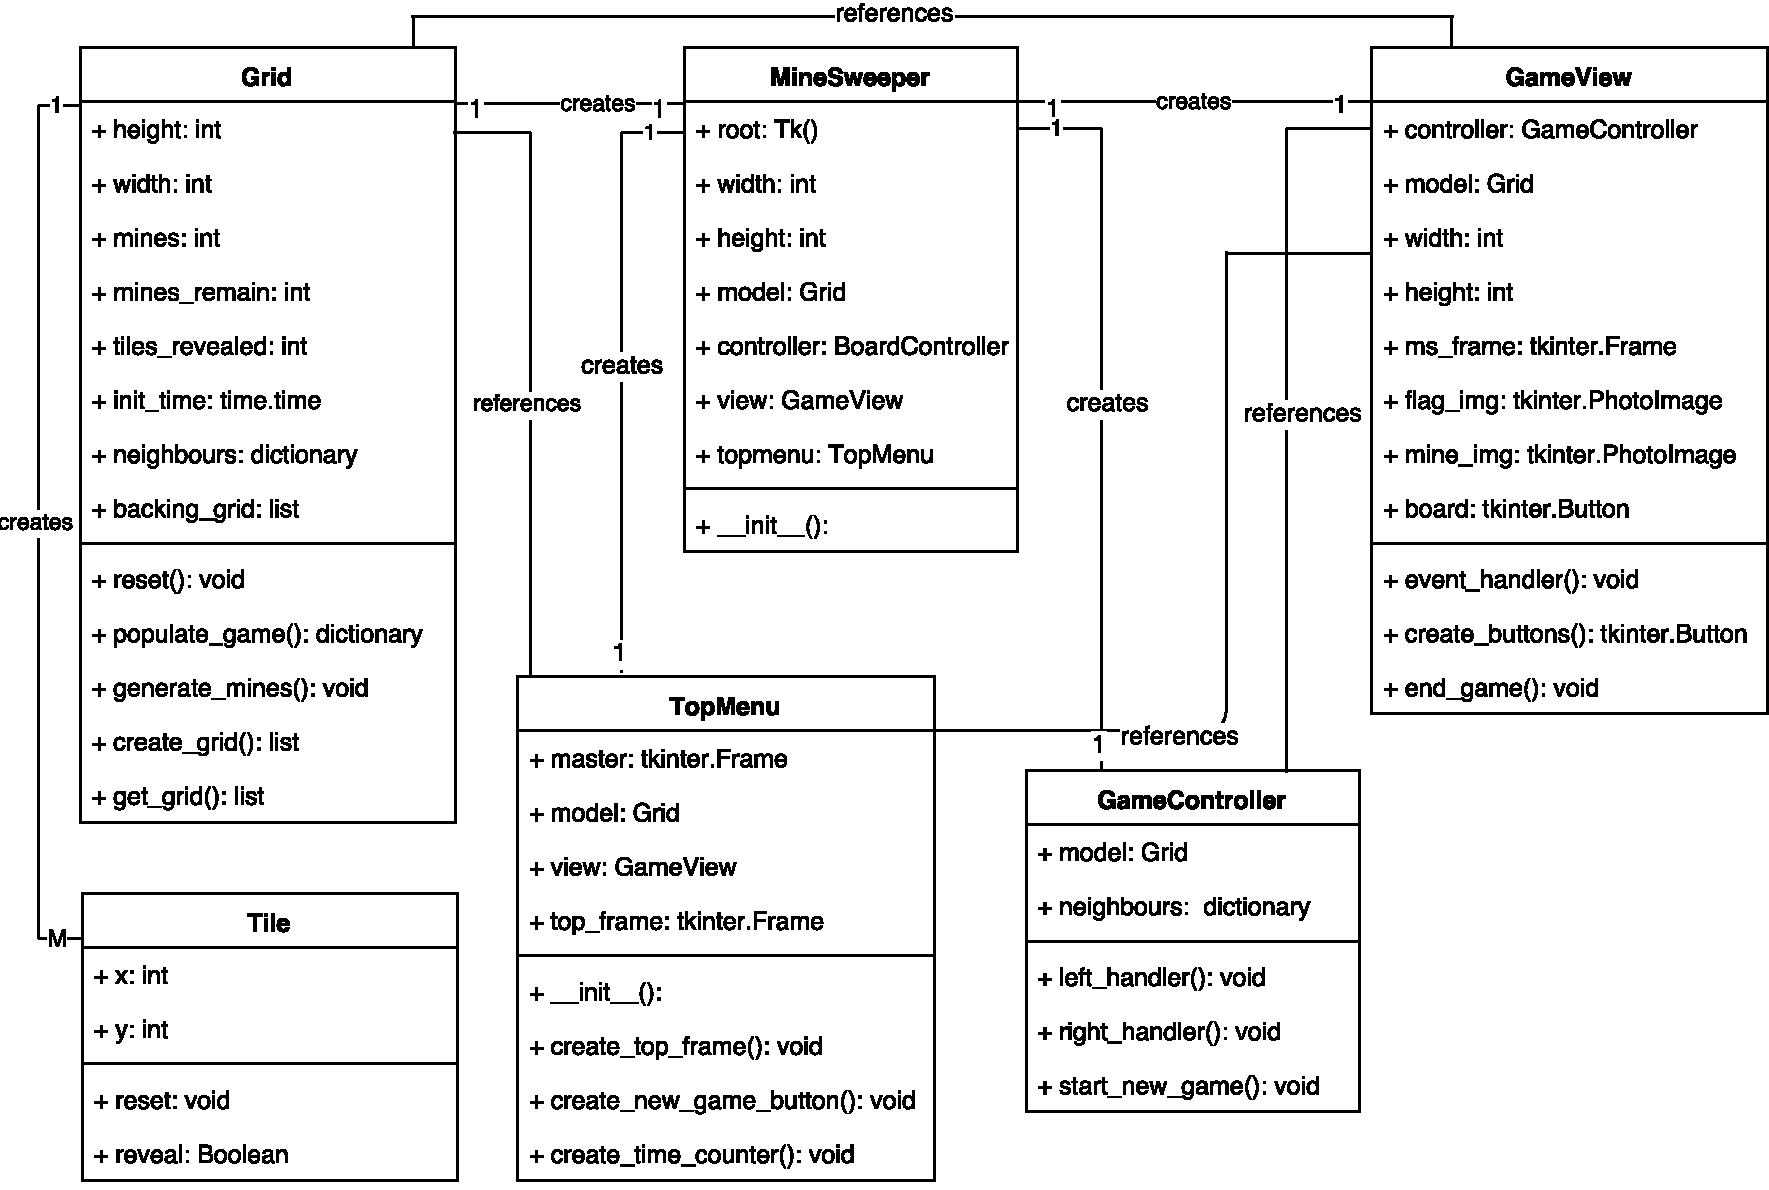
\includegraphics[scale=0.6]{UML}
		\caption{UML diagram for the Python implementation of MineSweeper}
	\end{figure}
\pagebreak
	
	\subsubsection{Software Patterns}
	
	
	\subsection{Testing}
	\par A software fault is a common occurence, a programmer makes an error, which results in a defect in the source code. Without testing with the intent for finding such  bugs, the program will produce the wrong outcome or results and cause it to fail. As soon as the program was executable, testing was conducted. The testing of Mine Sweeper took an agile approach as programming and testing needed to be done concurrently. The unittest module was imported in to the test file and unit tests were written to test separate functions of the program and as expected, some tests failed initially. Firstly, the populating of the game was tested - whether the information stored in the dictionary of neighbours was relative to the position of the mines. As the development of the program progressed, the written code passed incrementally larger portions of the test suites. The test suites are updated as new problems are found with the program. The unit tests are maintained along with the source code for Mine Sweeper. The goal of concurrently performing tests and writing the program ensures continuous integration. This also helps to meet the specified requirements of the software, makes sure the program responds accordingly to all kinds of user interaction and is sufficiently usable. This white-box style of software testing ensures that specific functions work as expected, especially for small pieces of software. Unit testing does not guarantee the functionality of the software alone however, it does ensure the building blocks of the software work independently from each other.
	
	
	\newpage

		\subsubsection{Version Control History / Log}
	\begin{tabular}{ | p{2cm} | p{13cm} | }
		\hline
		User & Activity \\
		\hline
		ZaymonFC & Finished testfile \\ 
		ZaymonFC & Merge branch 'master' of github.com/ZaymonFC/2810ICT\_Assignment \\ 
		ZaymonFC & Added diagrams and function description \\ 
		Natnicha & Added modifications to full system tests. \\ 
		Natnicha & Added more unit tests. \\ 
		ZaymonFC & Added system tests and put the main method contents of word ladder into a run function \\ 
		ZaymonFC & Added build test \\ 
		ZaymonFC & Merge conflict resolved \\ 
		ZaymonFC & Finished adding data structures and list of functions. \\ 
		Natnicha & Edited acceptance test and unit test in document. \\ 
		Natnicha & Merge branch 'master' of github.com/ZaymonFC/2810ICT\_Assignment \\ 
		Natnicha & Added unit tests to report. \\ 
		ZaymonFC & Added tests and added the banned words implementation to the word ladder \\ 
		ZaymonFC & Removed TestCase \\ 
		ZaymonFC & Added comments for some test cases in testfile.py \\ 
		ZaymonFC & Added multiple unit tests for different functions in word\_ladder \\ 
		ZaymonFC & Added tests for user input in testfile.py \\ 
		ZaymonFC & Logged work \\ 
		ZaymonFC & Fixed BFS and implemented a queue data type \\ 
		ZaymonFC & Added breadth first search for shortest path \\ 
		Natnicha & Resolved merge conflict \\ 
		Natnicha & Modified unit test section. \\ 
		ZaymonFC & Resolved merge conflict \\ 
		ZaymonFC & Added test skeleton for input validation \\ 
		Natnicha & Fixed spelling and name errors \\ 
		\hline 
	\end{tabular}
	
	\begin{tabular}{ | p{2cm} | p{13cm} | }
		\hline
		Natnicha & Merge branch 'master' of github.com/ZaymonFC/2810ICT\_Assignment \\ 
		Natnicha & Added requirement acceptance test \& user instructions. \\ 
		ZaymonFC & Added section describing all functions in the program \\ 
		ZaymonFC & Created UML and logical block diagrams, added to report \\ 
		ZaymonFC & Merge branch 'master' of github.com/ZaymonFC/2810ICT\_Assignment \\ 
		ZaymonFC & Modified test file and fixed formatting in report \\ 
		Natnicha & Merge branch 'master' of github.com/ZaymonFC/2810ICT\_Assignment \\ 
		Natnicha & Modified test table \\ 
		ZaymonFC & Fixed algorithm to find short paths by limiting reverse progress \\ 
		ZaymonFC & Merge branch 'master' of github.com/ZaymonFC/2810ICT\_Assignment \\ 
		ZaymonFC & Improved performance by reversing sorting direction of fitness function \\ 
		Natnicha & Added version control section \& Unit test tables \\ 
		Natnicha & Merge branch 'master' of github.com/ZaymonFC/2810ICT\_Assignment \\ 
		Natnicha & Added unittest cases \\ 
		ZaymonFC & Refactored word\_ladder.py to validate user input \\ 
		Natnicha & Modified listing for user requirements \\ 
		ZaymonFC & Added unittest file and added test ideas to README.md \\ 
		ZaymonFC & Added .gitignore file and removed postcompile latex objects \\ 
		ZaymonFC & Merge branch 'master' of github.com/ZaymonFC/2810ICT\_Assignment \\ 
		ZaymonFC & Modified report preamble to remove redundant packages \\ 
		Natnicha & Added headings and user requirements \\ 
		ZaymonFC & Added LaTeX template for assignment documentation \\ 
		ZaymonFC & Added program files and created project directory structure \\ 
		ZaymonFC & Initial Commit \\ \hline
		
	\end{tabular}
	
	\par\vspace{1cm}\small Note: Repository is private to prevent plagiarism. \textbar{} This log was created by using the command \begin{lstlisting} 
	git log --pretty=format:`%h;%an;%s' > ./log.csv\end{lstlisting}
	
	\pagebreak
	

	

\end{document}